\documentclass[sigconf]{acmart}

\usepackage{hyperref}

\usepackage{endfloat}
\renewcommand{\efloatseparator}{\mbox{}} % no new page between figures

\usepackage{booktabs} % For formal tables

\settopmatter{printacmref=false} % Removes citation information below abstract
\renewcommand\footnotetextcopyrightpermission[1]{} % removes footnote with conference information in first column
\pagestyle{plain} % removes running headers

\begin{document}
\title{Big Data and Artificial Intelligence Solutions for in Home, Community and Territory Security}


\author{Ashok Reddy Singam}
\orcid{HID337}
\affiliation{%
  \institution{Indiana University}
  \streetaddress{711 N Park Ave}
  \city{Bloomington} 
  \state{Indiana} 
  \postcode{47408}
}
\email{asingam@iu.edu}

\author{Anil Ravi}
\orcid{HID333}
\affiliation{%
  \institution{Indiana University}
  \streetaddress{711 N Park Ave}
  \city{Bloomington} 
  \state{Indiana} 
  \postcode{47408}
}
\email{anilravi@iu.edu}

\begin{abstract}
Having an intelligent ear-and-eye monitoring system at the home to constantly observe the surroundings both inside and outside can protect the house and personnel much more safer way. By extending this capability to the neighborhood and city through networking and collaboration would create safe cities across the world.

Anti-social activities became the most significant threat to national security because of their potential to bring massive damage to our homes, public infrastructure, economy, and people. The existing systems and methods haven't reached the level of sophistication to be able to consolidate the relevant data from variety of sources and demographics. Video surveillance of residential, commercial, military, and other restricted locations have been in practice since many years using various available technologies. Depending on the level of security, the data has been processed by data mining and/or big data analytics to take decisions by various personal, agencies and governments. However, the limitations of data collection, data mining and adoption of intelligence led to ineffective systems which are not predictive as they should be.The present security systems used by households are static cameras used at a  fixed location inside or outside the house. They are connected to network and provide alerts when any event occurred. However, they are not intelligent enough to understand the context, recognizing the people faces, and aware of family members behaviors, house needs etc.

With the advent of new technologies in Big Data and Artificial Intelligence fields, it possible to integrate the video, audio and social media data of targeted regions (homes, public places and extended areas) for security analysis. Such systems can use advanced statistical methods, classification algorithms and machine learning algorithms to predict and prevent the threats based on the severity probability.

\end{abstract}

\keywords{i523, HID333, HID337, Artificial Intelligence, Neural Networks, Machine Learning, Micro Drone}

\maketitle

\section{Introduction}
As per the book "Intelligence and Security Informatics"\cite{Kantor2005}, it is widely believed that information technology will play an indispensable role in making the world safer by supporting intelligence and knowledge discovery through collecting, processing, analyzing, and utilizing terrorism- and crime-related data. Social network analysis(SNA)has been widely explored to support intelligence and law enforcement agencies in investigating the terrorist and criminal social networks. It is valuable in identifying terrorists, suspect subgroups, and their communication patterns.

However, in the present world, the systems are disparately processing the data and the decisions/conclusions are being made without considering from multiple dimensions. The large corporations, nations, and intelligence agencies are using their individual systems but not taking integrated approach to solve the problems in their entirety. This could be due to political and economic interests of individuals, corporations and nations.

Analyzing the individual human behaviors, interactions, transactions, and actions is the key element in identifying the potential threat in advance. Generating and analyzing such data from individual homes and extending the concept to larger groups is the idea behind this research.

It is quite feasible to collect the data from individual homes and roll up to the communities, cities and then to the nations across the world. Since this involves with the personal data from people directly, it is required to follow privacy-preservation policies and methods enforced by local/national governments and law enforcement agencies. By accessing the lowest level of data of individuals video, voice, social media and other business transactional data would allow to characterize, analyze and assess the people behaviors and motives which can be maintained and processed as needed by Big Data systems. These systems are very complex in nature due to the variety, volume and velocity of the data, where the Big Data technologies will play a significant role in realizing them. In addition to data collection and mining, if artificial intelligence is applied to analyze and evaluate the data then the crime prediction and prevention would be feasible.

In order to realize such systems, one would need several technologies and sub-systems in various layers to effectively collect, transfer, mining, learning and analyze the data. In the following sections, it has been described some of the technologies/sub-systems that can be used to achieve the objectives of proposed conceptual model.
The discussion here consists of reviewing the available papers/systems related to security informatics and understanding the technologies and methods used. The gaps perceived in the review are attempted to solve by proposing a new concept. The remainder of this discussion is organized as follows:
\begin{itemize}
  \item Section 2 provides a set of sub-systems and use of them in the proposed framework. 
  \item Section 3 gives an overview community/city security using conceptual model. \item Finally, section 4 concludes this proposal.
\end{itemize}

\subsection{Data Collection}
As discussed in the above sections, the data can be collected from individual home level using the following means: video and voice enabled micro-drone, re-chargeable dock with edge processing server, WLAN (both infrastructure and Adhoc mode) with ability to transfer data to cloud server. This miniature sub-system hardware will have capability to harvest the large amounts of data from all major social media accounts of individual house mates such as Twitter, Facebook, YouTube, Instagram, WhatsApp, and Mobile Phone Calls and Texts and transfer to Big Data infrastructure. The Big Data infrastructure would organize the data through multiple data layers such as collection hub, staging hub and data lake.

\subsection{Data Privacy}
In the conceptual model that we have discussed, multiple sub-systems collect the individual home level information and uses anonymization models to preserve the privacy of individuals. The objective is hiding the sensitive personal information such as personal identities but publishing the rest of the data, an anonymized version of relational data. The data that will be sent out to be used for next level (community/region) fed to privacy preservation algorithms such as k-anonymity protection models which are being used in real-world systems known as Datafly, µ-Argus and k-Similar. The k-anonymity methods ensure that at least k records with respect to every set of quasi-identifier attributes are indistinguishable. There are other alternative methods such as l-diversity and m-invariance can be applied as well to apply different constraints on anonymity. For social network integration in to proposed system, models can use subgraph generalization approach to preserve the privacy, which has been discussed in the paper "Privacy-Preserved Social Network Integration and Analysis for Security Informatics"\cite{Yang2010}.

\subsection{Video Analytics}
The high quality video image frames will be processed to analyze the situational awareness. Learning hierarchical representation of video image data by using deep architecture models is the key component of video analytics. By using the deep learning algorithms to perform object detection, object tracking, face recognition, image classification and scene labeling would enable to establish a comprehensive situational awareness in the home security context. For example, facial expressions manifest not only emotions but also allied actions, behavioral patterns and give a lot of useful data when it comes to helping law enforcement and forensics agencies. Video Analytics can be achieved based on data curation, sentiment analysis, and other advanced solutions. Expressions like "happy", "sad", "angry", "scared", "surprised" or "neutral" form the basis of video analytics.

This method and approach can be extended to city and region levels by rolling up the data from individual homes. In the context of city and regional security, video analytics would help in people management, vehicle management, behavior monitoring. For example, in the public events deep learning enabled systems can  perform crowd detection, queue management, people counting, people scattering, people tracking; in the vehicle management, systems can perform vehicle classification, traffic monitoring, license plate recognition, road data gathering. Also, behavior monitoring can be achieved through motion detection, vandalism detection, face detection, privacy masking, and suspicious activity detection.
With the advent of new technologies in computing speed there are several Graphics Processing Units (GPU) integrated with high quality image sensors  introduced by technology companies such as NVidia can be used in the conceptual model. 

For example Pre-trained model of a region based convolutional neural networks (R-CNN) deployed on the Nvidia Jetson TX2 platform helps in recognizing and localizing objects like persons,cars, bikes etc.

\subsection{Voice Analytics}
The live voice recording integrated with video analysis provides better and accurate insight in to situation awareness for predicting and preventing the potential threats much faster. Traditional voice analytics tools rely on keywords and phonetics. These solutions are not well enough in deriving context and relevancy. With Big Data and AI advancements, now it is even possible to analyze for things like stress levels, lies, emotional content and more from audio data. Deep learning is becoming a mainstream technology for speech recognition and has successfully replaced Gaussian mixtures for speech recognition and feature coding at an increasingly larger scale. Google's Speech Recognition API built using deep learning neural network algorithms is one of the voice analytics software available in the market, which can be used in the proposed conceptual model.

\subsection{Social Media Analytics}
Security systems can be made more innovative and intelligent by integrating with social data. In the current world, social media like facebook,twitter,Instagram,watsapp etc are generating massive amounts of Big Data.If this information is used intelligently, it can predict behavior patterns and help to know about others.Typically, social analytics are used by marketing departments to predict the behavior and experience that consumers share in social networks. The same data can be used to monitor criminal activities.

\section{Home Security}
This section describes a proposed scalable security system building block concept, which can be extended to community, city and beyond.  The conceptual model has multiple sub-systems coordinate with each other to establish a robust home security system. In this model, a micro-drone integrated with video and audio will continuously monitor the house both inside and outside. An autonomous dual micro-drone model will have capability to view the surrounding with high resolution frame rates and transfer the data to edge processing unit and/or cloud based HDFS server. The social media data of housemates (e.g., E-mail, Facebook, Twitter, WhatsApp, and other web/mobile applications) gets integrated in to HDFS server.

This will establish a known context of complete information of individuals residing in-house by analyzing the contacts, communication exchange (phone calls, SMS, E-mails), trade transactions, and family/friends/foe information. With the combination of video, voice and social network data a comprehensive home security system can be achieved which not only protects the house but also individuals by having super knowledge about all the elements. This will require Big Data infrastructure along with machine learning algorithms in various sub-systems.

This conceptual model can be realized with available technologies and can be architected such that it will become a basic building block for scalable system.

\begin{figure}
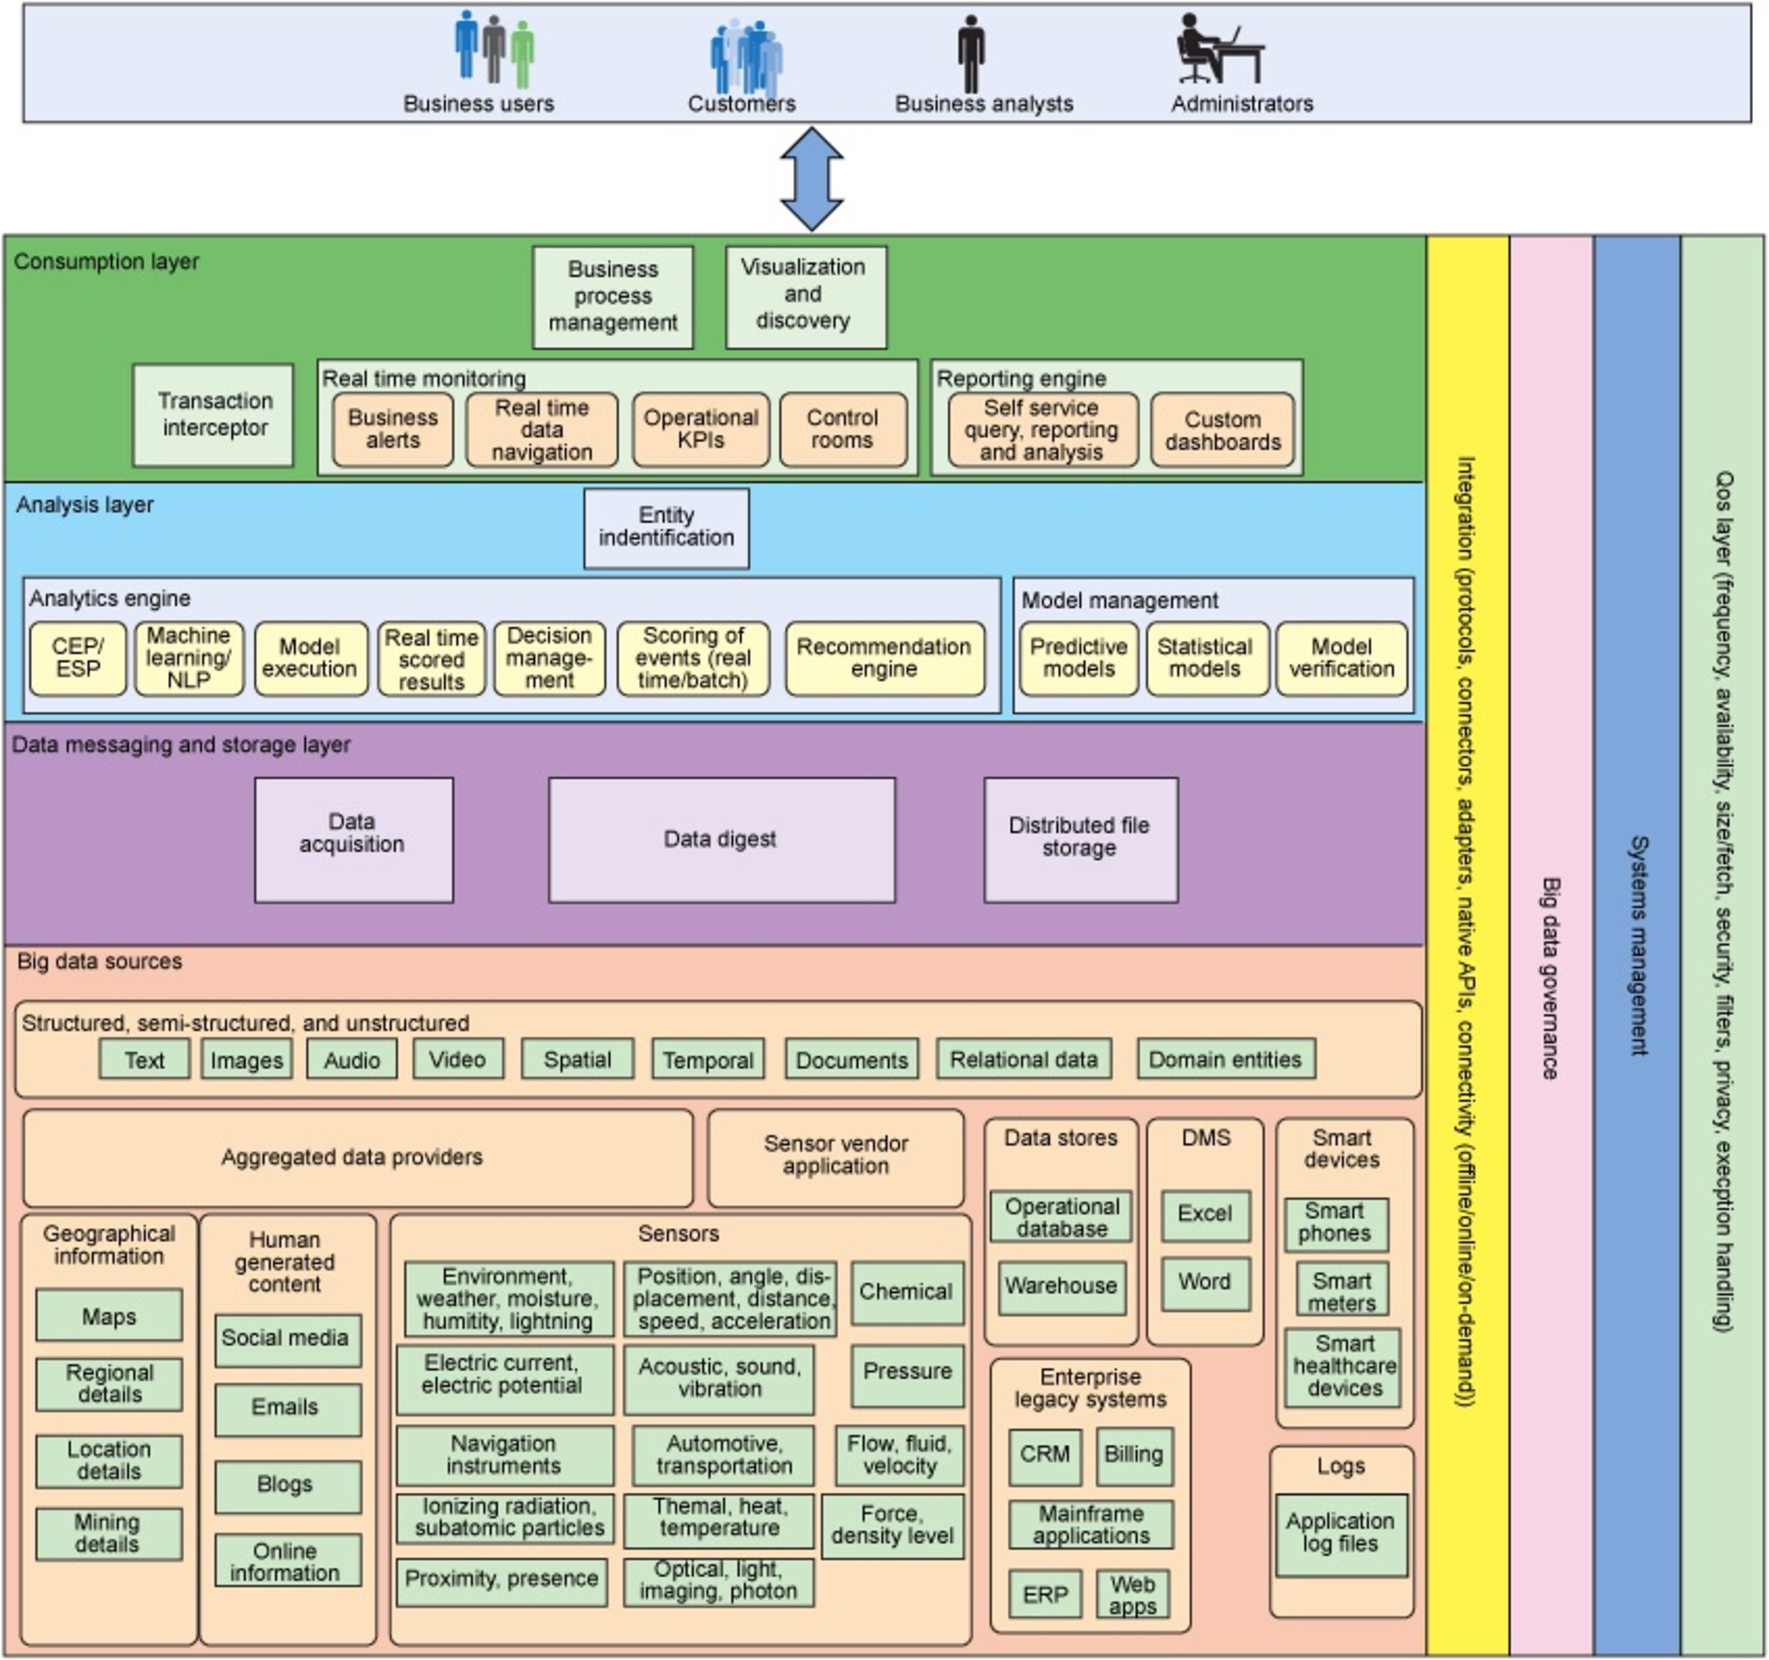
\includegraphics[height=7.5in, width=7.5in]{images/BigDataArchitecture.pdf}
\caption{Typical Big Data Architecture}
\end{figure}

\subsection{Dual Micro-Drones with Video and Audio}
The prevailing drone technology is reaching higher levels of sophistication allowing newer concepts to be realized in surveillance applications\cite{Labs2016}. In this proposed concept a micro-drone with integrated video, voice and environmental sensors (temperature, humidity, and accelerometers) can be designed along with learning algorithms to add intelligence. In the basic system, there will be two micro-drones to cover both in-side and out-side of the house (can consider adding more depending on the size of the house/facility) monitoring activities all the time. The drone hardware and software detects and recognize all moving objects through deep learning algorithms such as Regional Convolution Neural Networks (R-CNN). Li Wand and Dennis Sng\cite{Wang2015} have reviewed the recent progress of deep learning in object detection, object tracking, face recognition, image classification and scene labeling. The deep models have significantly improved the performance in these areas, often approaching human capabilities. The reasons for this success are two-folded. First, big training data are becoming increasingly available (e.g. data streams from a multitude of sensors) for building up large deep neural networks. Second, new advanced hardware (e.g. Nvidia GPUs) has largely reduced the training time for deep networks. 

The concept of micro-drone video and audio sub-system is to recognize human face and voice and establish the association. After the human object is created with face-voice association, the human characteristics, behaviors, social contacts, social media accounts, family/friends contact database and personal identification will be mapped. This person object (one of the housemate) will be constantly trained with large set of data during the learning period. Once the person object is matured with enough intelligence then the system will be ready for monitoring and analyzing the data of the person he/she actually mapped to. Multiple person objects will be created to map all the persons live in that house. The duo micro-drones are intelligent enough to recognize all the persons in the house and understand their behaviors, motives, actions, schedules, plans and their complete activities as time progresses.  

These micro-drones freely move around the house to monitor the family, friends, foes, strangers, and people who ever happen to be in the house surroundings and visit to meet housemates. Micro-drones are smart enough to sense the people emotions based on the expressions, conversations and actions to predict the immediate future consequences and get ready for protective actions (e.g., alerting appropriate people and agencies). Also, micro-drones are equipped with sensors to detect environment conditions (temperatures, wind, rain and humidity etc..,) to take good care of themselves by reaching back to dock/home stations while ensuring that security precautions are addressed. 
Since micro-drones are autonomous with self-maneuvering and self-diagnostics capabilities, they will take care of self-charging, protecting themselves from being damaged by staying away from objects and people reasonably.

The technologies available to realize such a micro-drone consists of: 
\begin{itemize}
  \item Autonomous octo/quadcopter 
  \item High resolution built-in 360 degree video cameras \item Finally, section 4 concludes this proposal
  \item High speed network links
  \item High speed GPUs
  \item Environment sensors
  \item Software with machine learning algorithms for various capabilities discussed in previous sections
\end{itemize}

\subsection{Learning Algorithms}
The two critical machine learning algorithms needed to realize the proposed concept are for the face and voice recognition. Deep learning models are potential candidates for these two tasks. Deep learning architectures have different variants such as Deep Belief Networks (DBN)\cite{Hinton2009}, Convolutional Neural Networks (CNN)\cite{NIPS2012_4824}, Deep Boltzmann Machines (DBM)\cite{pmlr-v9-salakhutdinov10a} and Stacked Denoising Auto-Encoders (SDAE)\cite{Vincent2010}, etc. The most attractive model is Convolutional Neural Networks which have achieved very promising results in both computer vision and speech recognition.

\subsection{Predictive Analysis }
The ability to estimate the occurrence of future events using expertise, observation and intuition is critical to the human decision-making process. From a biophysical perspective, there is strong evidence that the neocortex provides a basic framework for memory and prediction in which human intelligence emerges as a process of pattern storage, recognition and projection rooted in our experience of the world and driven by perception and creativity. There is increasing consensus among cognitive psychologists that human decision making can be seen as a situation-action matching process which is context-bound and driven by experiential knowledge and intuition.

\subsection{Community Drone Network}
The intelligent drone home security system would enable to provide comprehensive situational awareness at home level. The proposed drones are limited in their coverage area which is strictly enforced by regulatory/intelligence/government agencies. Since this inteli-drone is scalable to extend the coverage by just adding another device, it can be conceivable to create a network of inteli-drones to cover a given community. The community drone network is collection of security drones covering a specific region within a city which will ensure that relevant data is delivered to law enforcement and intelligence agencies. This would require one of the drones in the network to be nominated as \textit{Gateway Drone} to communicate with law enforcement/intelligence agencies. Each drone will have the capability to become a \textit{Gateway Drone} as needed. When the new drone is installed it will automatically look for existing \textit{Gateway Drone} in that community, which if exists then it will join the network and gets registered. If no \textit{Gateway Drone} is recognized, the new drone claims or becomes \textit{Gateway Drone}.

\section{City/Extended Regional Security}
The proposed conceptual model defines city level security network as a combination of multiple \textit{Community Drone Networks} together. In a given city there can be 'n' number of \textit{Community Drone Networks} based on the households, public places, and commercial entities. A network of \textit{Gateway Drones} forms as a \textit{City Drone Network} with one of the drones nominated as \textit{City Gateway Drone}.All the traditional networking principles can be applied to drone network as well with the \textit{Artificial Intelligence} enabled capabilities.
The information that will be routed from home-to-community-to-city-to-next level follows privacy preservation policies and law enforcement/intelligence agency regulations.

\section{Conclusions}
In this discussion, based on the review of existing literature, systems/products and technologies it has been perceived that security informatics systems are disparately implemented and consolidation of data and analysis at various layers hasn't been done efficiently. Considering that \textit{Big Data} technologies are robust enough to collect the large volumes of data from variety of sources, a conceptual model is proposed to discuss the feasibility of integrated video, voice, and social media data of individuals, communities and cities to be collected and analyzed to apply the learning algorithms. With the technologies such as high speed and parallel computing and Big Data infrastructure, machine learning algorithms can be applied to solve face and voice recognition. The combination of video, voice, and social network data the proposed conceptual system can address some of the prevailing home, community and territory security challenges and issues.

\begin{acks}
The authors would like to thank professor Gregor von Laszewski and his team for providing LaTex templates
\end{acks}

\bibliographystyle{ACM-Reference-Format}
\bibliography{report} 

\end{document}
